\documentclass[11pt,a4paper]{scrartcl}
\usepackage[utf8]{inputenc}
\usepackage[ngerman]{babel}
\usepackage{amsmath}
\usepackage{amsfonts}
\usepackage{amssymb}
\usepackage{lmodern}
\usepackage{paralist}
%\usepackage{titlepage}
\usepackage{tabularx}
\newcommand{\tablewidth}{.9\textwidth}
\setkomafont{sectioning}{\normalfont\normalcolor\bfseries}
\usepackage{graphicx}

\begin{document}
%\begin{fullsizetitle}
%	\centering
%	\vspace*{8cm}
%	\Huge
%	\scshape
%	Laborbericht zum Praktikum\par
%	\Large
%	Komplexe Informationstechnische Systeme\par
%	\vspace*{.5cm}
%	\large
%	Sommersemester 2016\par
%	\vspace*{2cm}
%	\normalfont\normalsize
%	Bennecke, Saskia\\
%	Clauß, Michael-Carsten\\
%	Lindner, Peter\par
%	\vspace*{5cm}
%	Technische Universität Ilmenau
%\end{fullsizetitle}
\section{Systemanalyse}
\subsection{Einleitung}
TODO: Allgemeines Blabla, wie der Versuch aufgebaut ist und was es so alles daran gibt, was gemacht werden soll... Ggf. mit nem Bildchen verfeinern.
\par %TODO 
Memos:
\begin{itemize}
	\item Richtungsangaben beziehen sich auf eine frontale Sicht auf den Aufbau, indem der Betrachter vor der Seite mit der Öffnung und der Kugelentnahmestation steht.
	\item Das korrekte Wort für die verschiedenfarbigen Teile der Scheibe lautet \glqq Sektor\grqq.
\end{itemize}
\subsection{Systemkomponenten}
Die mit dem Loch versehene Scheibe hat folgende Daten:
\begin{compactitem}
	\item Radius bis zum Loch: ca. 16\,cm\\
			(damit ergibt sich für die Lochbahn eine Länge von $2\pi\cdot16\text{\,cm} \approx 100$\,cm)
	\item Anzahl Sektoren: 12 (6 schwarze und 6 weiße, im Wechsel)\\
			(damit ergibt sich auf Lochhöhe die Länge des Sektorbogens zu $\frac{100\text{\,cm}}{12\text{\,cm}} = 8\frac{1}{3}\text{\,cm}$)
	\item Länge des Lochs: ca. 6\,cm
\end{compactitem}
\begin{table}[h]
	\centering
	\begin{tabularx}{\tablewidth}{|l|r|X|}
		\hline
		\bfseries Name & \bfseries Pin & \bfseries Beschreibung und Funktion\\\hline\hline
		Photosensor & 2 & Der Photosensor ist fest am Boden auf der hinteren rechten Seite des Aufbaus und erkennt, welche Art Kreissektor sich über ihm befindet:
		\begin{compactitem}
			\item \textbf{schwarzer Sektor:} Rückgabe $1$
			\item \textbf{weißer Sektor:} Rückgabe $0$
		\end{compactitem}
		\\\hline
		Hallsensor & 3 & Der Hallsensor ist fest am Boden auf der hinteren linken Seite des Aufbaus angebracht und erkennt anhand eines sich an der Scheibe befindlichen Magneten, wann das Loch an ihm vorbeikommt:
		\begin{compactitem}
			\item \textbf{Loch passiert Sensor:} setzt Wert ($1$)
			\item \textbf{Gegenseite passiert Sensor:} setzt zurück ($0$)
		\end{compactitem}
		Der Sensorwert wird also wieder auf $0$ gesetzt, wenn sich die Scheibe eine halbe Umdrehung weitergedreht hat.\\\hline
		Trigger & 4 & Der Trigger ist eine kleine kabelgebundene Fernbedienung mit einem Knopf. Der Sensorwert entspricht dem Knopfstatus:
		\begin{compactitem}
			\item \textbf{Knopf gedrückt:} Sensorwert $1$
			\item \textbf{Knopf nicht gedrückt:} Sensorwert $0$
		\end{compactitem}
		Zur Verdeutlichung: Für die konstante Ausgabe $1$ muss der Knopf gedrückt gehalten werden.
		\\\hline
	\end{tabularx}
	\caption{Sensorik}
\end{table}
\begin{table}[htbp]
	\centering
	\begin{tabularx}{\tablewidth}{|l|r|X|}
		\hline
		\bfseries Name & \bfseries Pin & \bfseries Beschreibung und Funktion\\\hline\hline
		Servomotor & 9 & Der Servomotor steuert die Freigabe von Kugeln aus dem Kugellager. Er dreht zeitgleich die zwei oben genannten Metallplättchen.\\\hline
	\end{tabularx}
	\caption{Aktorik}
\end{table}
\subsection{Messungen und Tests}
Memo:
\begin{compactitem}
\item Erwähnung des Fensters, für dass der Sensor gute Werte liefern muss (3,5 U/s bis 0,1 U/s)
\item Erwähnung Nyquist und Berechnung der passenden Frequenz
\item Erwähnung, dass das ne Schranke ist und wir aus Gründen 10 ms nehmen
\end{compactitem}
TODO %TODO
\subsection{Nutzung der Sensorwerte} \label{ssec:nutzung}
Um die geforderte Aufgabe umzusetzen, wurden zwei prinzipielle Möglichkeiten in Betracht gezogen, die sich auf die Art und Weise der verschiedenen Messvorgänge beziehen.
\paragraph{Möglichkeit 1: Polling} Für eine bestimmte Zeitdauer werden die Anzahl der Flankenwechsel gezählt, die der Photosensor liefert. Anhand dessen wird die Frequenz der Schwarz-Weiß-Wechsel gebildet und die Geschwindigkeit des Lochs auf der Bahn berechnet.
\begin{compactitem}
\item Die passende Wahl des Zeitintervalls der Messung ist problematisch, da das Ergebnis für ein breites Spektrum an Drehgeschwindigkeiten korrekt sein muss.
\item Ein festes Intervall muss sehr lang sein, da sehr langsame Drehungen richtig erkannt werden müssen.
\end{compactitem}
\paragraph{Möglichkeit 2: Interrupts} Nach Knopfdruck (Interrupt, dabei \#Knopfdrücke mitloggen) liefern die nächsten beiden Flanken des Photosensors ebenfalls einen Interrupt. Mittels einer einfachen binären Zustandsvariable wird das Warten auf die zweite Flanke realisiert. Nach der zweiten Flanke wird die Zeitdifferenz $\Delta t$ gebildet und anhand dessen die Geschwindigkeit $v_\text{Loch}$ des Lochs auf der Lochbahn: \[v_{\text{Loch}} = \frac{\text{Sektorbreite}}{\Delta t}\]

\section{Design}
	\newcommand{\class}[1]{\texttt{#1}}
\newcommand{\method}[1]{\texttt{#1}}
\newcommand{\attr}[1]{\textit{#1}}

Im Folgenden werden einige Designentscheidungen des Projekts beschrieben.
Dazu werden zuerst die entworfenen Klassen mit deren Attributen und Methoden beschriebenen.
Danach werden einige Verhaltensaspekte mit Sequenzdiagramm veranschaulicht.

\subsection{Struktur}
Diagramm \ref{fig:class_diagramm} zeigt alle Klassen des Projekts mit deren Beziehungen, Attributen und Methoden.


\begin{figure}[htbp]
	\centering
	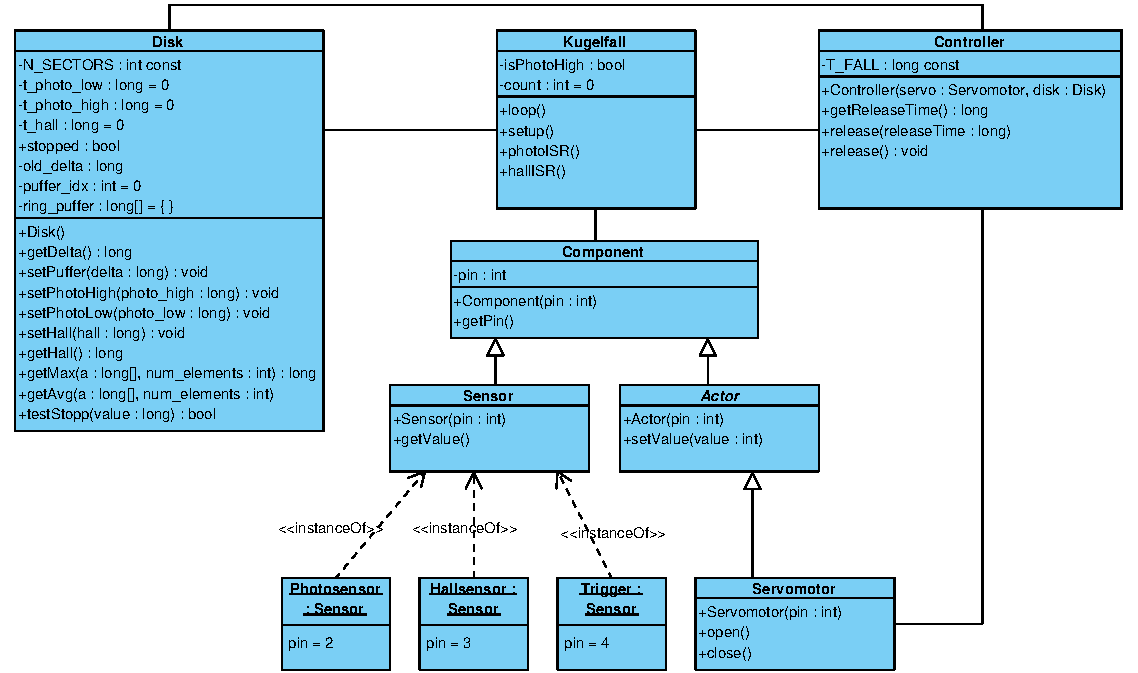
\includegraphics[width=\textwidth]{abb/class_cropped}
	\caption{Klassen mit deren Beziehungen, Methoden und Attributen}
	\label{fig:class_diagramm}
\end{figure}

\paragraph{\class{Kugelfall}}
ist die zentrale Klasse, da sie die Arduino-Methoden \method{setup()} und \method{loop()} enthält.
Sie steht in Beziehung zur allen anderen Klassen.
Innerhalb der \method{setup()}-Methode initialisiert sie die anderen Projekt-Klassen mit den entsprechenden Parametern (siehe Diagramm \ref{fig:setup_diagram}).
Ebenso werden die Interrupts zum Photosensor und Hallsensor mit den Methoden \method{photoISR()} bzw. \method{hallISR()} initialisiert (siehe Diagramm \ref{fig:photoISR} und \ref{fig:hallISR}).
Innerhalb der \method{loop()}-Methode wird auf Triggerdruck des Nutzers gewartet und ggf. der Mechanismus zur Berechnung der Fallzeit und das Loslassen aufgerufen (siehe Diagramm \ref{fig:loop_diagram}).

\paragraph{\class{Component}} entspricht einer Hardware-Komponente, auf welche mittels Arduino zugegriffen werden kann.
Es besitzt als einziges Attribut den \attr{pin} der Arduino-Komponente, welcher im Konstruktor initialisiert wird und mittels der Funktion \method{getPin()} abgerufen werden kann.

\paragraph{\class{Sensor}} entspricht einem Hardware-Sensor und ist eine Spezialisierung der Klasse \class{Component}. 
Es initialisiert die Instanz mit dem Pin-Modus \texttt{INPUT\_PULLUP} und dem übergebenen Pin.
Die Methode \method{getValue()} liest zur Aufrufzeit den entsprechenden Wert aus.
Dabei gibt es bei diesem Projekt insgesamt die drei Sensor-Exemplare \textit{Photosensor}, \textit{Hallsensor} und \textit{Trigger}, die jeweils mit den entsprechenden Pins initialisiert wurden. 

\paragraph{\class{Actor}} entspricht einem Hardware-Aktor und ist eine Spezialisierung der Klasse \class{Component}.
Es initialisiert die Instanz mit dem Pin-Modus \texttt{OUTPUT} und dem übergebenen Pin.
Die Methode \method{setValue()} schreibt den übergebenen Wert zum Aktor.

\paragraph{\class{Servomotor}} entspricht einem Hardware-Servomotor und ist eine Spezialisierung der Klasse \class{Actor}.
Es initialisiert im Konstruktur den Servomotor mit dem entsprechenden Pin.
Die Methoden \method{open()} und \method{close()} dienen zum Öffnen und Schließen des Servomotors und damit der Fallvorrichtung.

\paragraph{\class{Disk}} entspricht der Scheibe des Kugelfallaufbaus.
Neben festen Spezifikationen wie die Anzahl der Sektoren hat es auch die Attribute zum Festhalten der letzten Zeiten für Photosensor  (\method{setPhotoLow()}, \method{setPhotoHigh()}) und Hallsensor (\method{setHall()}). 
Zur Speicherung der Unterschiede der Zeitpunkte für steigende und fallende Flanke des Photosensor (Delta-Werte) nutzt es einen Ringpuffer, sodass die 24 zuletzt ermittelten Delta-Werte gespeichert werden (siehe Diagramm \ref{fig:photoISR}).
Zur Rückgabe eines Delta-Wertes (\method{getDelta()}) aus dem Ringpuffer wird die Funktion \method{getMax()} (bzw. \method{getAvg()}) verwendet.
So können Fehler aufgrund von Messungenauigkeiten kompensiert werden.
Die Funktion \method{computeSteadiness()} bestimmt, ob die Scheibe derzeit stabil oder nicht ist.
Dabei wird der aktuelle übergebene Delta-Wert mit dem vorherigen verglichen und im Falle eines großen Unterschiedes zwischen diesen beiden Werten wird die Scheibe als instabil angesehen.
Dieser Wert kann mit der Methode \method{isSteady()} ausgelesen werden.

\paragraph{\class{Controller}} dient zur Berechnung der Fallzeit und dem Loslassen der Kugeln.
So dient die Methode \method{waitForRelease()} zur der Berechnung Loslasszeit, dem Warten auf die korrekt Fallzeit und dann dem Loslassen (siehe Diagramm \ref{fig:loop_diagram}).
Zur Berechnung der Fallzeit dient die Methode \method{getReleaseTime()}, welche dabei die feste Fallzeit der Kugel \attr{T\_FALL}, einen dynamischen Delay (\method{getDynamicDelay()} und die Delta-Werte des Photosensors der Klasse \class{Disk} benutzt (näheres siehe Abschnitt \ref{ssec:nutzung}).
Für das Fallenlassen mit der Methode \method{release()} nutzt es die Klasse \class{Servomotor}.

\subsection{Verhalten}
Im Folgenden werden einige Verhaltensaspekte beschrieben.

Diagramm \ref{fig:setup_diagram} zeigt die Initialisierung der Anwendung mittels der Methode \method{setup} der Klasse \class{Kugelfall}.
\begin{figure}[htbp]
	\centering
	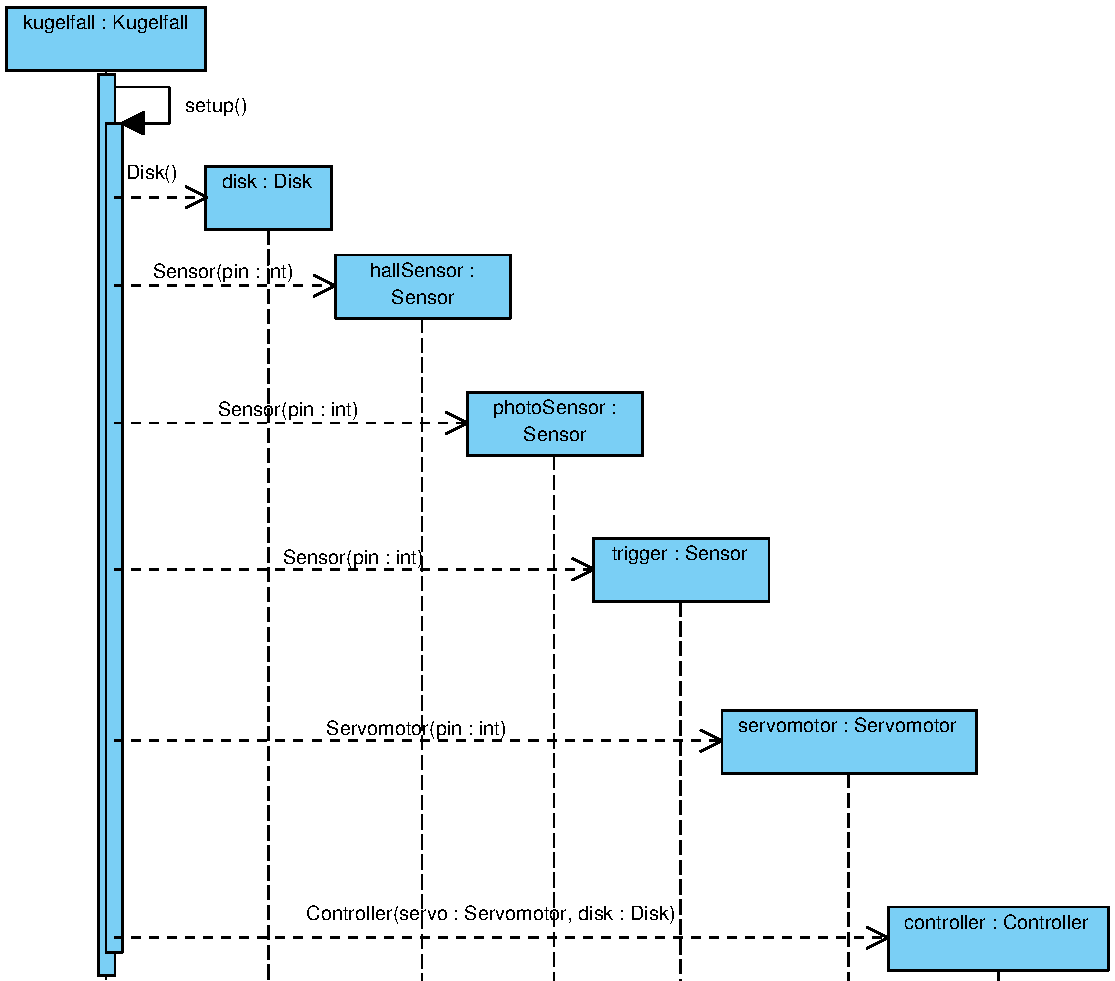
\includegraphics[width=\linewidth]{abb/setup_cropped}
	\caption{Ablauf bei der Methode \method{setup} von Klasse \class{Kugelfall}}
	\label{fig:setup_diagram}
\end{figure}
Dabei werden nacheinander die einzelnen Klassen instantiiert. 
Bei den Sensoren müssen die spezifischen Pins angegeben werden.
Bei der Initialisierung des \class{Controller} werden die Instanzen der Klassen \class{Servomotor} und \class{Disk} mit übergeben.

Diagramm \ref{fig:loop_diagram} zeigt auf sehr übersichtliche Art den Ablauf in der Dauerschleife in der Methode \method{loop()}.
\begin{figure}[htbp]
	\centering
	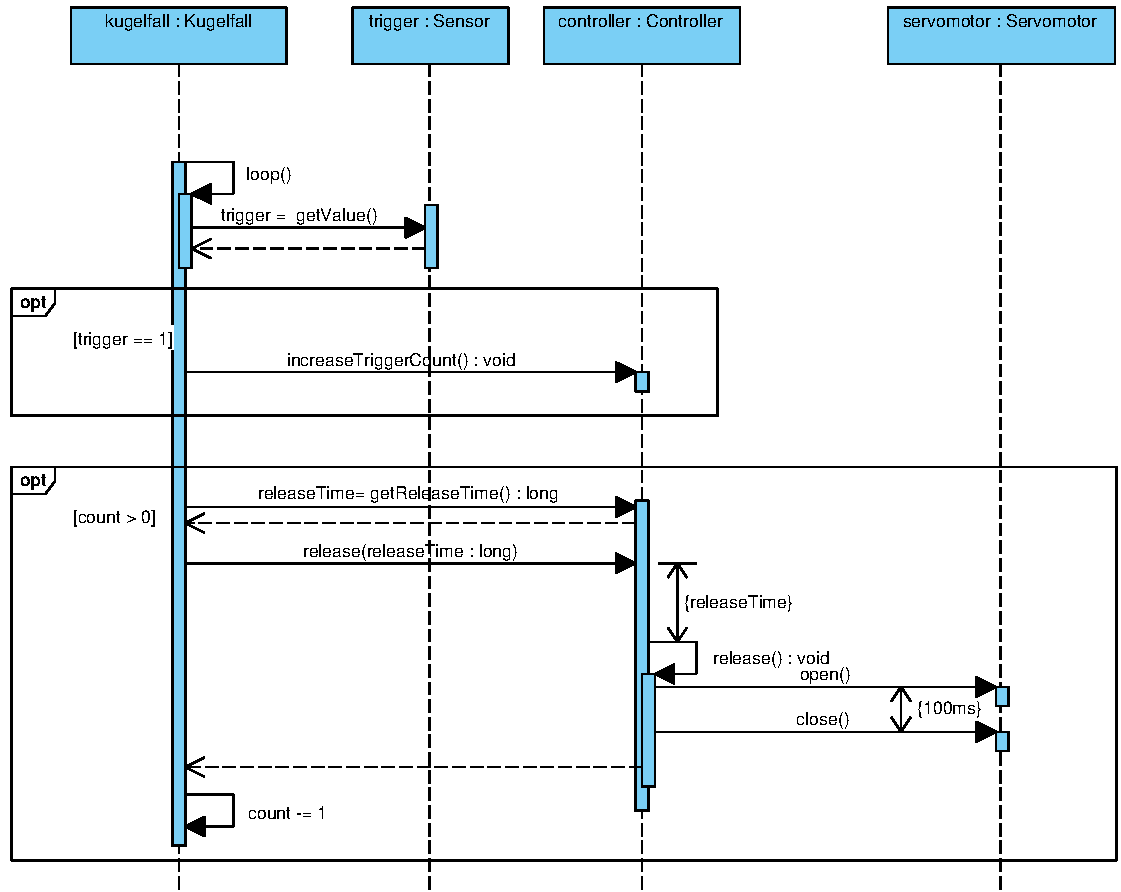
\includegraphics[width=\textwidth]{abb/loop_cropped}
	\caption{Ablauf bei der Methode \method{loop} von Klasse \class{Kugelfall}}
	\label{fig:loop_diagram}
\end{figure}
So wird zuerst der Triggerwert ausgelesen und damit geguckt, ob er vom Nutzer gedrückt wurde.
Ist das der Fall wird der Triggerzähler um eins erhöht.
Ist der Zähler derzeit größer null wird die Berechnung der Fallzeit und das Loslassen der Kugel mit der Methode \method{waitForRelease()} gestartet.
Dabei wird in der Dauerschleife zuerst mit der Methode \method{isSteady()} der Klasse \class{Disk} geprüft, ob sich die Scheibe derzeit stabil dreht.
Nur im Falle einer stabil drehenden Scheibe wird weiter fortgefahren.
So wird die mit der Methode \method{getReleaseTime()} die Zeit zum Loslassen der Kugel (näheres siehe Abschnitt \ref{ssec:nutzung}) und die aktuelle Zeit bestimmt.
Ist die Zeit bis zum Fallenlassen noch sehr lang ($>200$ms) wird die Schleife nochmals von vorne beginnen und somit auch die Loslasszeit aktualisiert.
Ist die Zeit bis zum Falllenlassen jedoch nur noch kurz ($\leq200$ms) wird mit Hilfe einer Dauerschleife solange gewartet, bis die richtige Zeit erreicht ist und mit der Methode \method{release()} losgelassen.
Zum Loslassen der Kugel werden die Methoden der Klasse \class{Servomotors} verwendet.
Nach dem Loslassen wird der Triggerzähler wieder verringert.
Das Vorgehen mit der Fallunterscheidung in Hinblick auf die verbleibende Zeit hat den Vorteil, dass die Zeit im Falle einer weit entfernten Loslasszeit nochmals aktualisiert wird, sodass jedwede Veränderungen, welche durch die Verlangsamung der Scheibe auftreten können, berücksichtigt werden.

Diagramm \ref{fig:photoISR} zeigt den Ablauf zum Festhalten der Messwerte des Photosensor mittels \method{photoISR()}. 
\begin{figure}[htbp]
	\centering
	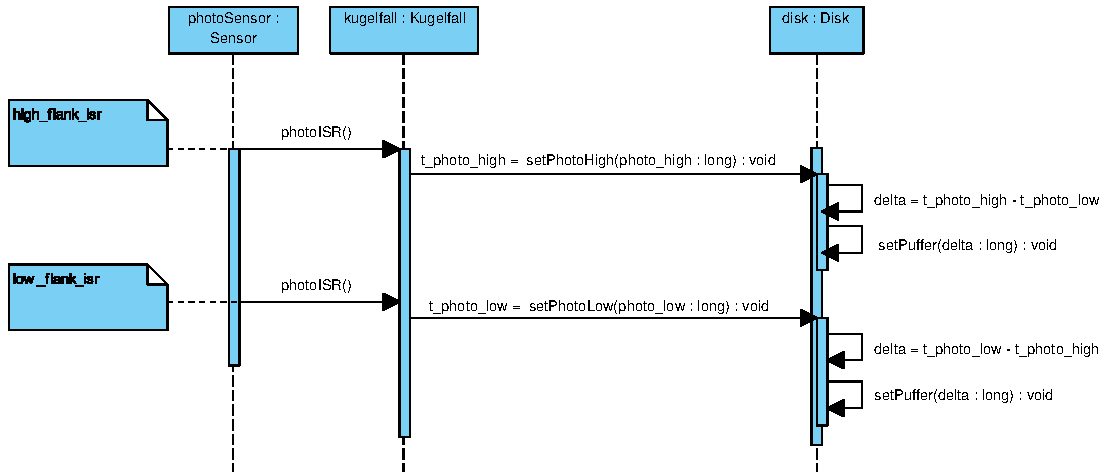
\includegraphics[width=\textwidth]{abb/photoISR_cropped}
	\caption{Ablauf bei der Methode \method{photoISR} von Klasse \class{Controller}}
	\label{fig:photoISR}
\end{figure}
So wird die  Methode \method{photoISR()} in Folge von steigenden und fallenden Flanken des Photosensor aufgerufen.
Die Werte mittels der Methode \method{setPhotoHigh()} bzw. \method{setPhotoLow()} gesichert.
Dabei wird zuerst die Differenz der Werte berechnet und diese dann mit der Methode \method{setPuffer()} innerhalb des Ringpuffers gespeichert.
%Zur Unterscheidung der steigenden und fallenden Flanken dient die boolesche Variable \attr{isPhotoHigh}.

%Denn es stehen mit diesem Ringpuffer nicht nur auf der letzte Wert, sondern die letzten 20 Werte zur Verfügung.

Diagramm \ref{fig:hallISR} zeigt den Ablauf zum Festhalten der Messwerte des Hallsensor mittels \method{hallISR()}.
\begin{figure}[htbp]
	\centering
	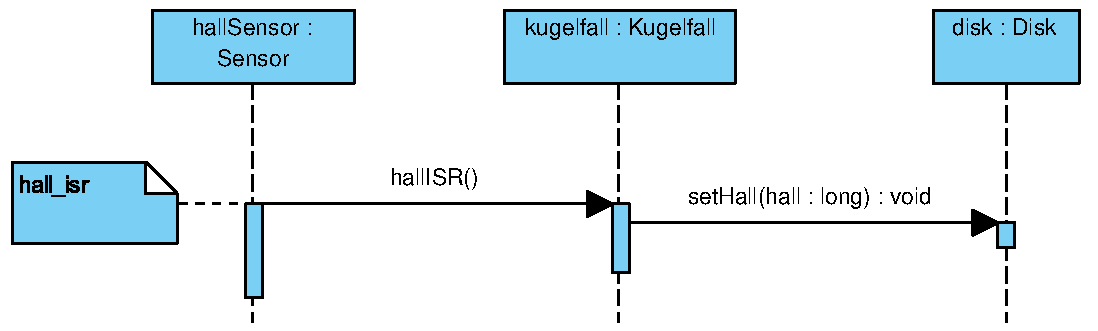
\includegraphics[width=0.8\textwidth]{abb/hallISR_cropped}
	\caption{Ablauf bei der Methode \method{hallISR} von Klasse \class{Controller}}
	\label{fig:hallISR}
\end{figure}
So wird die Methode \method{hallISR()} in Folge einer steigenden Flanke aufgerufen und die Werte Mittels der Method \method{setHall()} gespeichert.
Der aktuelle Wert kann mittels \method{getHall()} ausgelesen werden.

\end{document}